%! TeX program = lualatex
\section{Introduction}
\frenchspacing

\begin{frame}
  \frametitle{Whad do we want to achieve?}
    From various sources (HTML, ePub) create PDF suitable for various outputs:
    \begin{itemize}
      \item e-book readers
      \item smartphones or tablets
      \item various print page formats
    \end{itemize}

  \end{frame}
  \begin{frame}
    \frametitle{Why?}

    \begin{itemize}
      \item comfortable reading
      \item archiving
      \item because we can
    \end{itemize}


\end{frame}

\section{How do we convert HTML to PDF for an e-reader?}

\begin{frame}
  \frametitle{Rmodepdf}

  A script that converts  web pages to PDF.

  \begin{itemize}
    \item extracts clean text from articles, without ads and navigation elements on the pages
    \item should allow configuration for individual websites or e-book editions (e.g., MK Prague)
    \item configurable output
  \end{itemize}

  % Work in progress code is located here:

  \url{https://github.com/michal-h21/rmodepdf/}
\end{frame}

\begin{frame}
  \frametitle{Page with control elements and ads}
  \begin{center}
    
\includegraphics[height=.9\textheight]{img/root-balast.png}
  \end{center}
\end{frame}

\begin{frame}
  \frametitle{Page in reader mode}
  \begin{center}
    \includegraphics[height=.9\textheight]{img/root-čtečka.png}
  \end{center}
\end{frame}

\begin{frame}
  \frametitle{Reader mode for scripts}
  Reader mode is a feature in web browsers that removes control elements from the page and displays only the article text.

  \bigskip

  \begin{tabular}{ll}
    Readability.js & \url{https://github.com/mozilla/readability}\\
    Python-readability & \url{https://github.com/buriy/python-readability}\\
    Rdrview: & \url{https://github.com/eafer/rdrview}\\
  \end{tabular}

\end{frame}


\begin{frame}
  \frametitle{How do we load and transform HTML files?}
  LuaXML contains two libraries for HTML processing and transforming
  \begin{itemize}
    \item LuaXML contains a Transform library for converting XML to other formats, such as \TeX
      \begin{itemize}
        \item allows rules for specific elements selected using CSS selectors
      \end{itemize}
    \item the DOM library can now load HTML files
  \end{itemize}
\end{frame}

\section{Rmodepdf usage}


% \begin{frame}
%   \frametitle{What's next?}
%   \begin{itemize}
%   \item automate the design of the output document for different display sizes
%   \item automatically prevent typesetting errors:
%     \begin{itemize}
%       \item widows and orphans
%       \item line breaks with single-letter prepositions, units, or academic titles
%       \item overflow lines when typesetting narrow columns
%     \end{itemize}
%   \end{itemize}
% \end{frame}


\section{Responsive Design in \LaTeX}

\begin{frame}
   \frametitle{What is Responsive Design}
   \begin{itemize}
     \item flexible structure - adjusting the size of elements on the page to the display device
     \item media queries - rules applied based on the properties of the display device (screen size, type of display, etc.)
   \end{itemize}

   Thanks to these features, the same page code can be well displayed both on a large monitor and on mobile devices.
\end{frame}

\begin{frame}
  \frametitle{Page Example on a Large Monitor}
  \begin{center}
    
\includegraphics[height=.9\textheight]{img/pedf-web-big.png}
  \end{center}
\end{frame}

\begin{frame}
  \frametitle{Page Example on a Small Screen}
  \begin{center}
    \includegraphics[height=.9\textheight]{img/pedf-web-small.png}
  \end{center}
\end{frame}

\begin{frame}
  \frametitle{The \texttt{responsive} Package}

  A package inspired by responsive design methods for web pages
  \begin{itemize}
  \item adjusting font size to display size
  \item typographic scale for font sizes
  \item media queries
  \end{itemize}
  \url{https://github.com/michal-h21/responsive-latex}
    % - changes in the number of characters per line
    % - margins using newgeometry
\end{frame}

\begin{frame}[fragile]
  \frametitle{Setting Font Size Based on Display Size}

  Font size can be set using the command \verb|\setsizes{number of characters per line}|.
  
\begin{columns}
  \begin{column}{0.5\textwidth}
\begin{verbatim}
\begin{minipage}{5cm}
\setsizes{25}

\lipsum[1]

\end{minipage}
\end{verbatim}
\end{column}
\begin{column}{0.5\textwidth}

\fbox{%
\begin{minipage}{5cm}
\ResponsiveSetup{lineratio=38}
\setsizes{25}

\normalsize

Lorem ipsum dolor sit amet,
consectetuer adipiscing elit.
Ut purus elit, vestibulum ut,
placerat ac, adipiscing vitae,
felis. 

\end{minipage}}
\end{column}
\end{columns}

\end{frame}

\begin{frame}[fragile]
  \frametitle{Difference in Font Size Based on Number of Characters}
\begin{columns}
  \begin{column}{0.5\textwidth}
\begin{verbatim}
\setsizes{55}
\end{verbatim}

\fbox{%
\begin{minipage}{5cm}
\setsizes{55}

\lipsum[1]

\end{minipage}}
\end{column}
\begin{column}{0.5\textwidth}
\begin{verbatim}
\setsizes{25}
\end{verbatim}

\fbox{%
\begin{minipage}{5cm}
\ResponsiveSetup{lineratio=38}
\setsizes{25}

\normalsize

Lorem ipsum dolor sit amet,
consectetuer adipiscing elit.
Ut purus elit, vestibulum ut,
placerat ac, adipiscing vitae,
felis. 

\end{minipage}}
\end{column}
\end{columns}
\end{frame}

\begin{frame}[fragile]
  \frametitle{Configuration}
  Options can be set when calling the package or later using the command \verb|\ResponsiveSetup|.

  Important options:

  \begin{description}
    \item[noautomatic] -- do not set font size automatically at the beginning of the document
    \item[characters] -- number of characters when automatically setting the font size
    \item[scale] -- typographic scale used for font sizes
    \item[lineratio] -- ratio used when calculating line height
  \end{description}

\end{frame}

\begin{frame}[fragile]
  \frametitle{Line Height}
  Line height can be influenced by the \texttt{lineratio} option. 
The higher its value, the smaller the distance between lines.

\begin{columns}
  \begin{column}{0.5\textwidth}
\begin{verbatim}
\ResponsiveSetup{lineratio=38}
\end{verbatim}

\fbox{%
\begin{minipage}{5cm}
\ResponsiveSetup{lineratio=38}
\setsizes{65}

\lipsum[1]

\end{minipage}}
\end{column}
  \begin{column}{0.5\textwidth}
\begin{verbatim}
\ResponsiveSetup{lineratio=34}
\end{verbatim}

\fbox{%
\begin{minipage}{5cm}
\ResponsiveSetup{lineratio=34}
\setsizes{65}

\lipsum[1]

\end{minipage}}
\end{column}
\end{columns}
\url{https://www.smashingmagazine.com/2020/07/css-techniques-legibility/}

\end{frame}

\newcommand\printsize[1]{\csname #1\endcsname\par\noindent Sample\par}
\newcommand\showscale[2][.5\textwidth]{%
      % \setsizes[38]{25}
      \printsize{huge}
      \printsize{LARGE}
      \printsize{Large}
      \printsize{large}
      \hrule
      \printsize{normalsize}
      \hrule
      \printsize{small}
      \printsize{footnotesize}
}

\begin{frame}[fragile]
  \frametitle{Font Styles}

  The sizes of individual font styles are chosen based on the typographic scale

\begin{columns}
  \begin{column}{0.5\textwidth}
Default scale (pentatonic)

\fbox{%
\begin{minipage}{5cm}
\setsizes{45}

\showscale{}

\end{minipage}}
\end{column}
  \begin{column}{0.5\textwidth}
\begin{verbatim}
\ResponsiveSetup{scale=golden}
\end{verbatim}

\fbox{%
\begin{minipage}{5cm}
\ResponsiveSetup{scale=golden}
\setsizes{45}

\showscale

\end{minipage}}
\end{column}
\end{columns}
\url{https://spencermortensen.com/articles/typographic-scale/}

\end{frame}

\begin{frame}[fragile]
  \frametitle{Finer Scale Adjustment}

  We can also directly set the ratio and number of steps by which the scale increases by this ratio.

\begin{columns}
  \begin{column}{0.5\textwidth}
\begin{verbatim}
\ResponsiveSetup{ratio=2,
number=2,scale=none}
\end{verbatim}

\fbox{%
\begin{minipage}{5cm}
\ResponsiveSetup{ratio=2,
number=2,scale=none}
\setsizes{45}

\showscale{}

\end{minipage}}
\end{column}
  \begin{column}{0.5\textwidth}
\begin{verbatim}
\ResponsiveSetup{ratio=1.3,
number=2,scale=none}
\end{verbatim}

\fbox{%
\begin{minipage}{5cm}
\ResponsiveSetup{ratio=1.3,
number=2,scale=none}

\setsizes{45}

\showscale

\end{minipage}}
\end{column}
\end{columns}

\end{frame}

\begin{frame}[fragile]
\frametitle{CSS Media Query Example}
\begin{verbatim}
body {
  color: green;
}
@media screen and (max-width: 600px) {
    body {
      color: blue;
    }
}
\end{verbatim}
\end{frame}
          
\begin{frame}[fragile]
  \frametitle{Media Queries in \LaTeX}
    Using the \verb|\mediaquery| command, we can test various properties:
  
    \begin{itemize}
  \item physical page size
  \item line length
  \item page orientation
\end{itemize}

Additional tests can be easily added.

\end{frame}

\begin{frame}[fragile]

  \frametitle{Media Query Example}

  This example displays fewer characters if the text width is less than 4 cm.

\begin{verbatim}
\mediaquery{max-textwidth=4cm}
{\setsizes{45}}{\setsizes{60}}
\end{verbatim}
\begin{columns}
  \begin{column}{0.5\textwidth}

\fbox{%
\begin{minipage}{5cm}
\mediaquery{max-textwidth=4cm}
{\setsizes{45}}
{\setsizes{60}}

\lipsum[1]

\end{minipage}}
\end{column}
  \begin{column}{0.5\textwidth}

\fbox{%
\begin{minipage}{3.9cm}
\mediaquery{max-textwidth=4cm}
{\setsizes{45}}
{\setsizes{60}}

\lipsum[1]

\end{minipage}}
\end{column}
\end{columns}

\end{frame}

\begin{frame}
  \frametitle{Do Media Queries Make Sense in \LaTeX?}
  \begin{itemize}
    \item possibly in universal packages
    \item using different templates for different sizes is easier
  \end{itemize}
\end{frame}

\section{Automatic Typesetting}

\begin{frame}
  \frametitle{\texttt{lua-widow-control} Package}
  Suppression of widows and orphans using Lua callbacks
  \begin{itemize}
    \item Each paragraph is typeset twice -- once with normal parameters, the second time with one extra line
    \item The impact on speed should be minimal
    \item If an orphan is found, the previous paragraph is replaced with the version with the extra line
  \end{itemize}
  \url{https://ctan.org/pkg/lua-widow-control}
\end{frame}

\begin{frame}
  \frametitle{Example of an Orphan}
  \begin{center}
    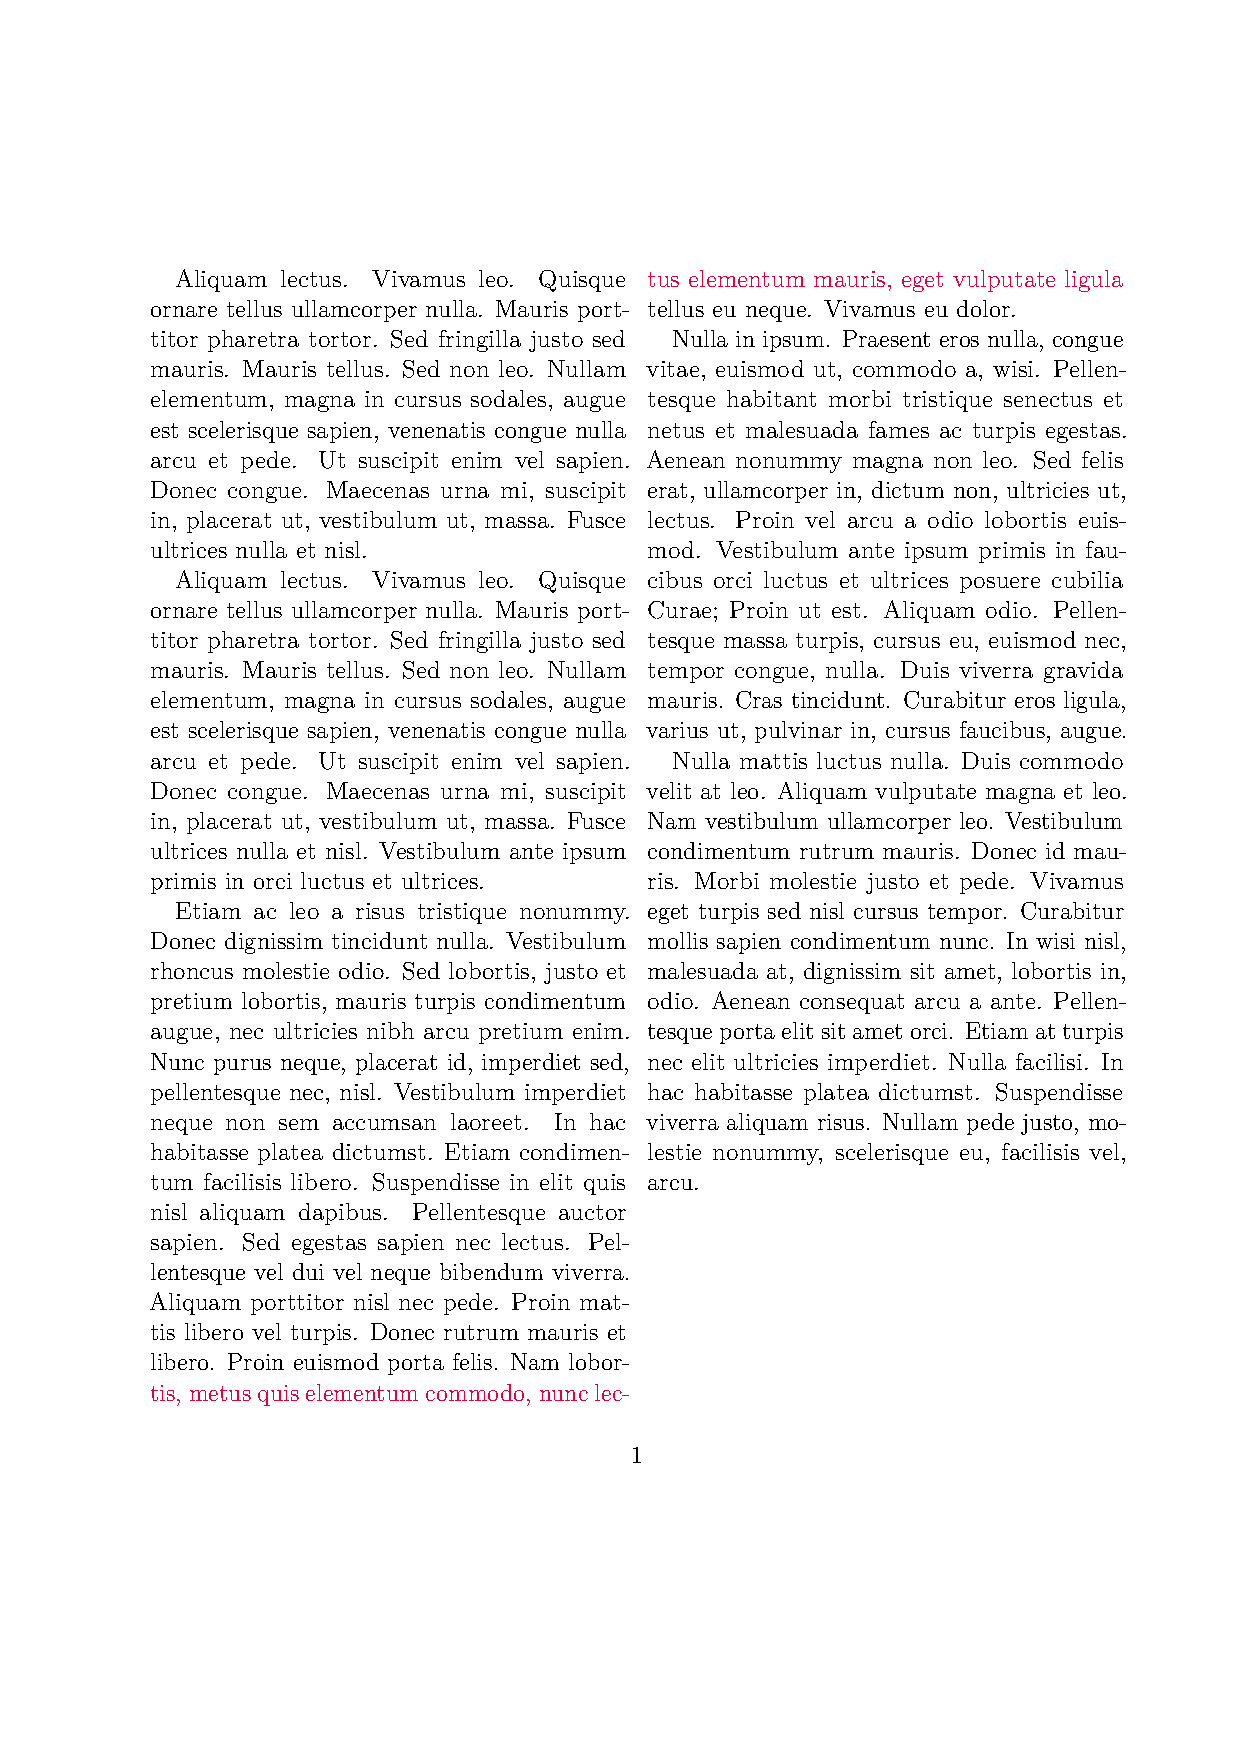
\includegraphics[height=\textheight,page=1]{examples/widow.pdf}
  \end{center}
\end{frame}

\begin{frame}
  \frametitle{Suppressed Orphan}
  \begin{center}
    \includegraphics[height=\textheight,page=2]{examples/widow.pdf}
  \end{center}
\end{frame}

\begin{frame}
  \frametitle{Comparison of Different Methods to Reduce Orphans}
  \begin{priklad}
  \begin{center}
  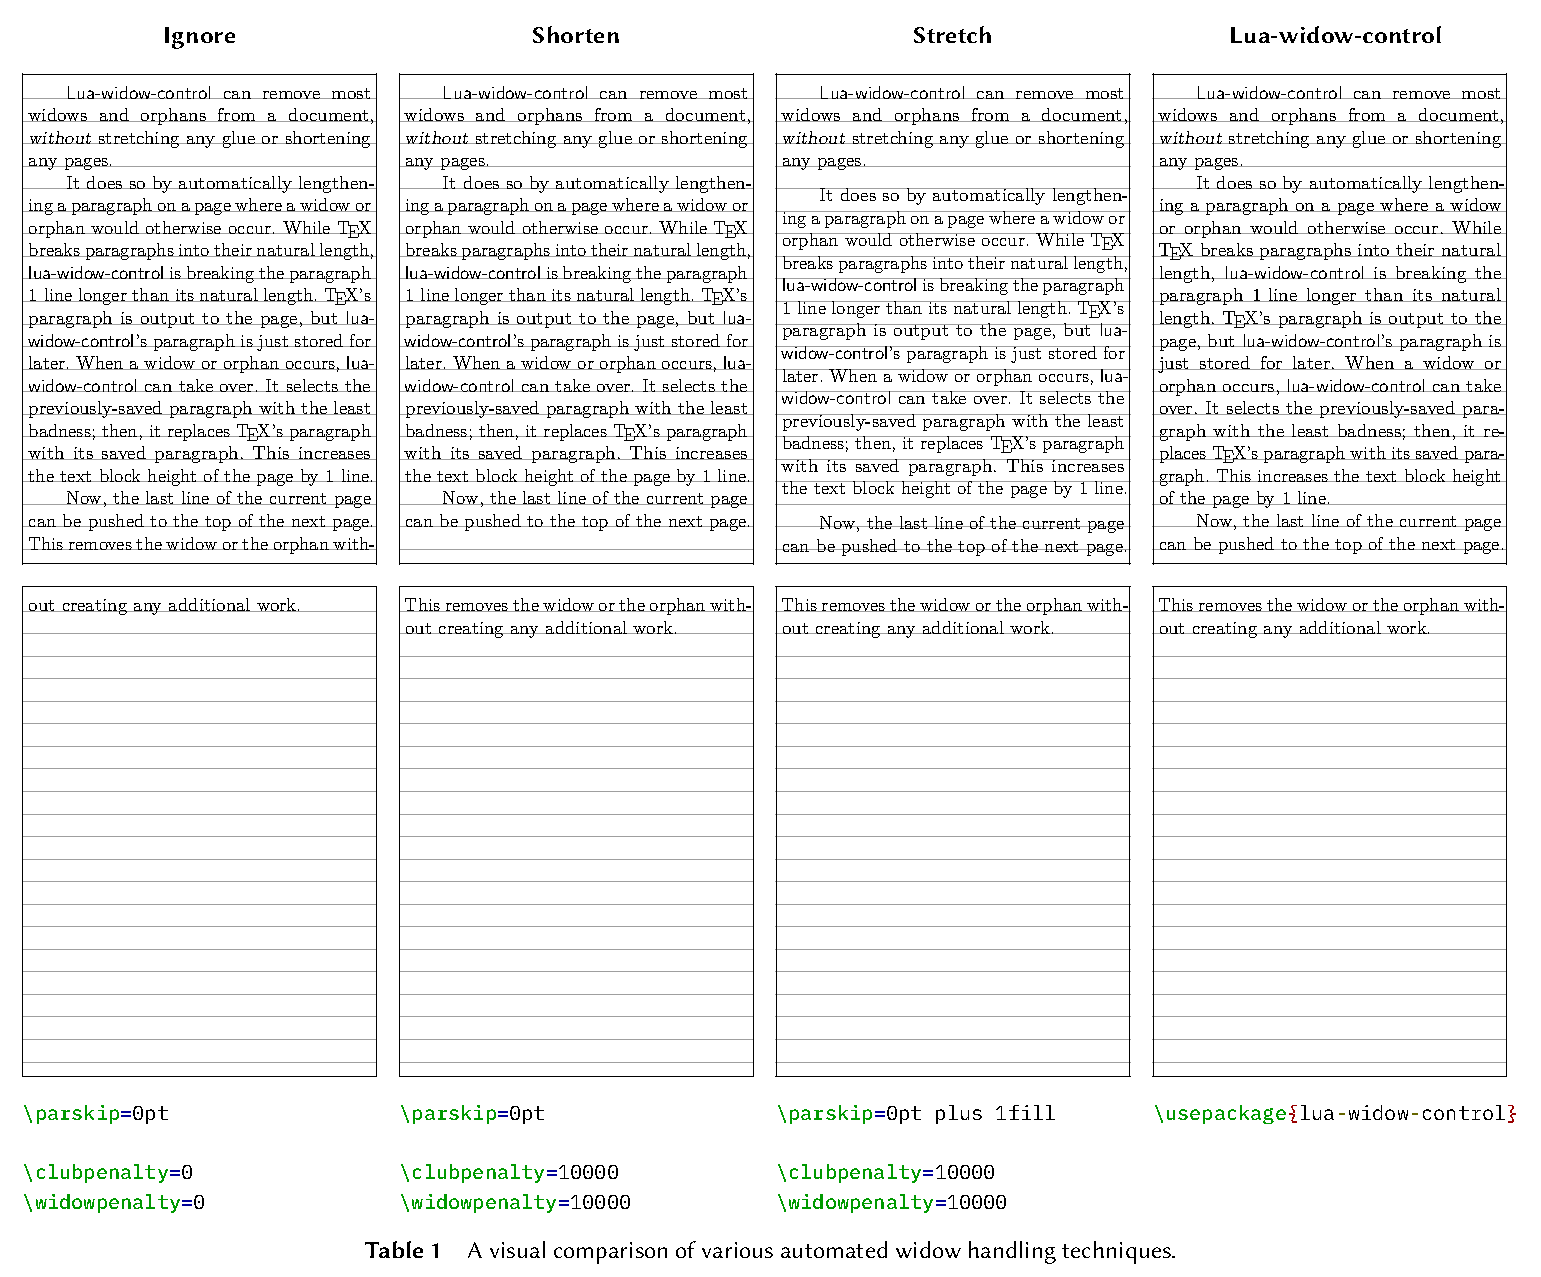
\includegraphics[height=.95\textheight]{img/lua-widow.pdf}
  \end{center}
  \end{priklad}
  % \myfig[height=0.8\textheight]{img/lua-widow.pdf}{}
\end{frame}

\begin{frame}[fragile]
  \frametitle{Configuration Options}
 \begin{verbatim}
 \lwcsetup{...}
 \end{verbatim}
 \begin{description}
   \item[default] -- does not add any vertical spaces but may lead to overly airy paragraphs
   \item[strict] -- primarily uses vertical spaces and does not create bad paragraphs,  
     \begin{itemize}
       \item but only removes a third of orphans
       \item works poorly mainly for documents that contain only text, fiction, etc.
     \end{itemize}
   \item[balanced] -- combines both methods, removes 90\% of orphans
  \end{description}
\end{frame}

\begin{frame}[fragile]
  \frametitle{Limitations}
    \begin{itemize}
      \item \verb|\clubpenalty| and \verb|\widowpenalty| have no effect, and can even cause side effects
      \item Support for multi-column typesetting is limited, the Multicol package does not work
  \end{itemize}
\end{frame}

\begin{frame}[fragile]
  \frametitle{\texttt{luavlna} Package}
    Prevents line breaks:
      \begin{itemize}
        \item After single-word prepositions
        \item At initials
        \item At academic titles
        \item Between numbers and units
      \end{itemize}
  \url{https://ctan.org/pkg/luavlna}
\end{frame}

\begin{frame}
  \frametitle{Usage Example of Luavlna}
  \begin{minipage}{3in}

    \preventsingledebugon

    Text with short consonants and vowels and other phenomena
    from the range of possibilities (possible in text).

    How about characters with diacritics?

    Various possibilities [in brackets \textless and other characters

    Support for initials and titles: M. J. Hegel, Ing. Běháková, Ph.D., Ž. Zíbrt,
    Ch. Borner.

    Support for units: 100.5 MN\cdot{}s, 100.5 kJ, 200 µA, $-1$ dag, 1 MB. 1 kJ.

    Inside mathematics, processing should be disabled: $k \in \mathbb N$.

    \preventsingledebugoff
  \end{minipage}
\end{frame}

\begin{frame}
    \frametitle{Hyphenation of Compound Words}
    \begin{center}
    \begin{minipage}{2in}
      Sedlec-Prčice, blue-green, translator-interpreter, cook-waiter, propane-butane, Otýlie Sklenářová-Malá, František Jílek-Oberpfalcer.
    \end{minipage}
  \end{center}
\end{frame}

\begin{frame}
  \frametitle{Package Options}
  Using options, we can disable certain features
  \begin{description}
    \item [noprocess] – do not process the document automatically
    \item [noinitials] – initials
    \item [nounits] – SI units
    \item [nopredegrees] – titles before the name
    \item [nosufdegrees] – titles after the name
  \end{description}
\end{frame}

\begin{frame}[fragile]
  \frametitle{Useful Commands}
  \begin{itemize}
    \item \verb|\singlechars{language}{letters}| -- list of letters for which line breaking is suppressed
    \item \verb|\enablesplithyphens{language}| -- sets support for hyphenation of compound words for the given language
    \item \verb|\preventsinglelang{language}| -- sets the rules for the given language for the entire document
  \end{itemize}
\end{frame}

\begin{frame}[fragile]
  \frametitle{Supported Languages}
  Built-in support is only for Czech and Slovak:

\begin{verbatim}
\singlechars{czech}{AIiVvOoUuSsZzKk}
\singlechars{slovak}{AIiVvOoUuSsZzKk}
\end{verbatim}

The language needs to be selected using the Babel or Polyglossia packages

\begin{verbatim}
An example in Czech.
\selectlanguage{english}
An example in English.
\end{verbatim}

    \preventsingledebugon

An example in Czech.
\selectlanguage{english}
An example in English.

    \preventsingledebugoff

    \selectlanguage{czech}

\end{frame}

\newcommand\testbox[1]{%
  \parbox{150pt}{%
    \parindent=15pt%
    \tolerance=1%
    \pretolerance=1%
    #1
  }%
}

\newcommand\printtest[1]{%
  \linebreakerdisable%
  \noindent\testbox{%
    #1
    \par\medskip\noindent\hfill\textbf{Without Linebreaker}\hfill\null
  }%
  \linebreakerenable%
  \hfill%
  \testbox{%
    #1
    \par\medskip\noindent\hfill\textbf{With Linebreaker}\hfill\null
  }%
}

\begin{frame}[fragile]
  \frametitle{\texttt{linebreaker} Package}
  Prevents the occurrence of overfull lines
  \begin{itemize}
    \item Affects only the typesetting of paragraphs where such a line occurs
    \item If it detects an overfull line in a paragraph, it retypesets it with larger values for
      \verb|tolerance| and \verb|emergencystretch|.
  \end{itemize}
  \url{https://ctan.org/pkg/linebreaker}
\end{frame}

\begin{frame}
  \frametitle{Example}
  \printtest{
    The example document given below creates two pages by using Lua code alone. You
will learn how to access TeX's boxes and counters from the Lua side, shipout a
page into the PDF file, create horizontal and vertical boxes (hbox and vbox),
create new nodes and manipulate the nodes links structure. 
%The example covers the following node types: rule, whatsit, vlist, hlist and action.
  }
\end{frame}

\begin{frame}[fragile]
  \frametitle{Configuration}
  Linebreaker can be configured using the \verb|\linebreakersetup| command:
  \begin{description}
    \item[maxcycles] -- number of attempts to retypeset a paragraph
    \item[maxemergencystretch] -- maximum value of \verb|\emergencystretch|
    \item[maxtolerance]  -- maximum value of \verb|tolerance|
  \end{description}
\begin{verbatim}
\linebreakersetup{
maxtolerance = 90,         % default 9999
maxemergencystretch = 1em, % default 3em
maxcycles = 4              % default 30
}
\end{verbatim}

\end{frame}

% \section{Conclusion}

\begin{frame}[standout]
  Thank you for your attention!

  \url{michal.h21@gmail.com}

  \url{www.kodymirus.cz}
\end{frame}


